% =========================================================
% Openness vs Completeness (Conceptual Distinction)
% =========================================================

\subsection{Openness vs Completeness}
\label{sec:openness-vs-completeness}

\subsubsection{Definitions and Core Ideas}

\begin{definition}[Open Set]
Let $(X,d)$ be a metric space and let $U \subseteq X$.
The set $U$ is \emph{open} if
\[
\forall x \in U \;\exists r>0 \text{ such that } B(x,r) \subseteq U .
\]
\end{definition}

\begin{definition}[Complete Metric Space]
A metric space $(X,d)$ is \emph{complete} if every Cauchy sequence in $X$
converges to a point of $X$.
\end{definition}

\begin{remark}
Although both concepts arise early in analysis, they describe
very different properties of a space.
\end{remark}

\paragraph{Openness is Local.}

The definition of openness says that every point of the set
has a small neighborhood contained entirely inside the set.

\[
\boxed{\text{Openness = local room around each point}}
\]

The condition only concerns what happens in a small neighborhood of
each individual point.

\paragraph{Completeness is Global.}

Completeness describes what happens to infinite processes,
specifically limits of sequences.

\[
\boxed{\text{Completeness = limits of Cauchy sequences exist in the space}}
\]

This property concerns the structure of the space as a whole.

\subsubsection{Consequences and Conceptual Takeaways}

\begin{remark}[Local vs Global Structure]
Many theorems about open sets rely only on local properties
and therefore hold in any metric space, even if the space
is not complete.

For example, the following are true in every metric space:

\begin{itemize}
\item Arbitrary unions of open sets are open.
\item Finite intersections of open sets are open.
\end{itemize}

These results depend only on the definition of open ball,
not on completeness.
\end{remark}

\begin{example}[Openness in an Incomplete Space]
Consider the metric space $(\mathbb{Q},|\cdot|)$.
This space is not complete.

The set
\[
U = (-1,1) \cap \mathbb{Q}
\]
is open in $\mathbb{Q}$.

Every rational number $x$ with $|x|<1$ has a small interval
of rational numbers around it contained in $U$.

Thus openness does not require completeness.
\end{example}

\begin{remark}[Mental Model]
A useful way to remember the distinction is:

\[
\textbf{Openness: every point has breathing room.}
\]

\[
\textbf{Completeness: limits have somewhere to land.}
\]
\end{remark}

% =========================================================
% Pathological Open Sets
% =========================================================

\subsection{Pathological Open Sets}
\label{sec:pathological-open-sets}

One of the important lessons of topology and analysis is that
open sets can have extremely complicated shapes.
The definition of openness depends only on local neighborhoods,
not on the global geometry of the set.

\subsubsection{The Comb Example}

Define the subset $C \subseteq \mathbb{R}^2$ by
\[
C =
\left(
\bigcup_{n=1}^{\infty}
\{(1/n,y) : 0 \le y \le 1\}
\right)
\cup
\{(0,y) : 0 \le y \le 1\}.
\]

Geometrically this set looks like a comb:

\begin{itemize}
\item infinitely many vertical ``teeth'' at $x = 1/n$
\item a vertical ``spine'' at $x=0$
\end{itemize}

Now consider the complement
\[
U = \mathbb{R}^2 \setminus C .
\]

\begin{proposition}
The set $U$ is open in $\mathbb{R}^2$.
\end{proposition}

\begin{remark}
Even though the set $C$ contains infinitely many slits that
accumulate near $x=0$, every point of the complement still
has a small ball that avoids these slits.
Thus the complement remains open.
\end{remark}

\subsubsection{A Set with Infinitely Many Holes}

Another instructive example is the following subset of $\mathbb{R}$.

Define
\[
U = (0,1) \setminus
\bigcup_{n=1}^{\infty}
\left(
\frac{1}{3^{\,n+1}}, \frac{2}{3^{\,n+1}}
\right).
\]

This construction removes infinitely many small intervals
from $(0,1)$.

The removed intervals accumulate toward $0$,
producing infinitely many holes at smaller and smaller scales.

\begin{remark}
Despite the infinitely many holes,
the resulting set is still open.

Each point that remains has a small interval around it
contained entirely in the set.
\end{remark}

\subsubsection{Why These Examples Matter}

These examples illustrate several key ideas:

\begin{itemize}
\item Open sets can have extremely irregular geometry.
\item The concept of openness depends only on local neighborhoods.
\item The global appearance of a set does not determine whether it is open.
\end{itemize}

Thinking about such examples helps prepare the intuition needed
for later subjects such as:

\begin{itemize}
\item General topology
\item Measure theory
\item Fractal geometry
\item Functional analysis
\end{itemize}

In all of these areas, sets can be far more complicated than
the simple intervals and disks encountered in elementary calculus.




% =========================================================
% TikZ: Topologist's Comb (the "comb set")
% C = ( ⋃_{n≥1} {1/n}×[0,1] ) ∪ ({0}×[0,1]) ∪ ([0,1]×{0})
% (Often the base segment [0,1]×{0} is included in the classic picture.)
% =========================================================

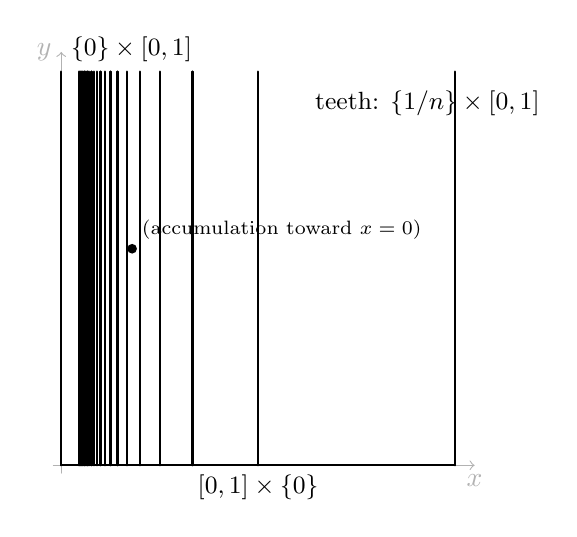
\begin{tikzpicture}[scale=5, line cap=round, line join=round]

  % Axes (optional)
  \draw[->, gray!60] (-0.02,0) -- (1.05,0) node[below] {$x$};
  \draw[->, gray!60] (0,-0.02) -- (0,1.05) node[left] {$y$};

  % Base segment [0,1] x {0}
  \draw[thick] (0,0) -- (1,0);

  % Spine {0} x [0,1]
  \draw[thick] (0,0) -- (0,1);

  % Teeth at x = 1/n, n=1..N
  \def\N{22}
  \foreach \n in {1,...,\N} {
    \pgfmathsetmacro\x{1/(\n)}
    \draw[thick] (\x,0) -- (\x,1);
  }

  % Labels
  \node[above right] at (0,1) {\small $\{0\}\times[0,1]$};
  \node[below] at (0.5,0) {\small $[0,1]\times\{0\}$};

  \node[anchor=west] at (0.62,0.92) {\small teeth: $\{1/n\}\times[0,1]$};

  % Optional: a point showing accumulation near x=0
  \fill (0.18,0.55) circle (0.35pt);
  \node[above right] at (0.18,0.55) {\scriptsize (accumulation toward $x=0$)};

\end{tikzpicture}


